\documentclass[12pt]{article}
\usepackage{amsmath}
\usepackage{amssymb}
%\usepackage{hyperref}
\usepackage{epsfig,graphicx,amsmath}
\usepackage{amsfonts}
\usepackage{enumerate}
\usepackage{amsfonts}
\usepackage{amssymb}
\usepackage{amsthm}

%%%%%%%%%%%%%%%%%%%%%%%%%%%%%%%%%%%%%%%%%%%%%%%%%%%%%%%%%%%%%%%%
\newcommand{\mb}[1]{\mbox{\boldmath$#1$}}
\newcommand{\p}{\partial}
\newcommand{\ds}{\displaystyle}
\newcommand{\beq}{\begin{eqnarray}}
\newcommand{\beqq}{\begin{eqnarray*}}
\newcommand{\eeq}{\end{eqnarray}}
\newcommand{\eeqq}{\end{eqnarray*}}
\newcommand{\eps}{\varepsilon}
\newcommand{\erf}{\mbox{erf}}
\newcommand{\erfi}{\mbox{erfi}}
\newcommand{\Ei}{\mbox{Ei}}
\newcommand{\x}{\mbox{\boldmath$x$}}
\newcommand{\Aa}{\mbox{\boldmath$A$}}
\newcommand{\rr}{\mbox{\boldmath$r$}}
\newcommand{\As}{\mbox{\boldmath$a$}}
\newcommand{\y}{\mbox{\boldmath$y$}}
\newcommand{\z}{\mbox{\boldmath$z$}}
\newcommand{\J}{\mbox{\boldmath$J$}}
\newcommand{\ET}{\mbox{\boldmath$\eta$}}
\newcommand{\n}{\mbox{\boldmath$n$}}
\newcommand{\X}{\mbox{\boldmath$X$}}
\newcommand{\Y}{\mbox{\boldmath$Y$}}
\newcommand{\Yy}{\mbox{\boldmath$y$}}
\newcommand{\Z}{\mbox{\boldmath$Z$}}
\newcommand{\w}{\mbox{\boldmath$w$}}
\newcommand{\vv}{\mbox{\boldmath$v$}}
\newcommand{\bb}{\mbox{\boldmath$b$}}
\newcommand{\Bb}{\mbox{\boldmath$b$}}
\newcommand{\B}{\mbox{\boldmath$B$}}
\newcommand{\ALPHA}{\mbox{\boldmath$\alpha$}}
\newcommand{\aaa}{\mbox{\boldmath$a$}}
\newcommand{\C}{\mbox{\boldmath$C$}}
\newcommand{\SSigma}{\mbox{\boldmath$\Sigma$}}
\newcommand{\mmu}{\mbox{\boldmath$\mu$}}
\newcommand{\IIm}{\mbox{\boldmath$I_m$}}
\newcommand{\mean}[1]{\langle #1\rangle}
\newcommand{\diffunit}{$\mu$m$^2$.s$^{-1}$}
\newcommand{\Li}{\mbox{Li}}
\newcommand{\thet}{\mbox{\boldmath$\theta$}}
\newcommand{\intR}{\int\limits_{\mathbb{R}}}
\newcommand{\intRm}{\int\limits_{\mathbb{R}^m}}
\newcommand\norm[1]{\left\lVert#1\right\rVert}
%\definecolor{red}{rgb}{1,0,0}

\usepackage{color}
\usepackage{float}
\begin{document}	
\title{ Material and methods}
\maketitle
%%%%%%%%%%%%%%%%%%%%%%%%%%%%%%%%%%%%%%%%%%%%%%%%%%%%%%%%%%%
\section{Modeling  histones redistribution following UV damages}
%%%%%%%%%%%%%%%%%%%%%%%%%%%%%%%%%%%%%%%%%%%%%%%%%%%%%%%%%%%
We present here a coarse-grained model for nucleosomes and chromatin re-organization following UV damages. At steady-state, nucleosomes are modeled as fixed beads located on the chromatin, itself modeled as a one dimensional unstructured wire. We use the model to study the relaxation of the chromatin and nucleosomes to a steady state, measured after 15 minutes.
%%%%%%%%%%%%%%%%%%%%%%%%%%%%%%%%%%%%%%%%%%%%%%%%%%%%%%%%%%%
\subsection{Dynamics of histones following UV damages in the region of interest ROI}
%%%%%%%%%%%%%%%%%%%%%%%%%%%%%%%%%%%%%%%%%%%%%%%%%%%%%%%%%%%
Following the experimental protocol, the initial damage circular region (IDR) induced by the laser beam is centered around the focal point (origin of the coordinates), with an exposure time $u \in [5-100]$ ms. Following this laser induction, because the tagged damages point region increases and reaches a plateau at 15 minutes, this domain is defined as the region of interest ROI (see also the empirical definition in XXX) and our goal is to estimate the amount of DNA and nucleosomes that has left this region. We assume that the loss of DNA and nucleosomes is due to two mechanisms: one is nucleosome sliding along the chromatin and outward in the direction of the ROI boundary and the second is chromatin expansion or unfolding. First, the nucleosomes involved in sliding are those that contained damaged DNA wrapped around them. In this model, a nucleosome cannot detach from the chromatin or pass through another one. The exact mechanism of motion is not considered here because we will only consider the steady-state final position, defined at 15 min post UVC. Note that there is no limitation in the distance that they can slide. In second mechanism, nucleosome and DNA are lost in equal proportion due to DNA unwrapping (Fig. 3XXX). Note that due to expansion of chromatin, the DNA and nucleosome located in the annulus between the ROI and IDR is going to be extruded from the ROI.

In the model, due to the radial symmetry, we consider that chromatin is a single wire of total length $l$, with one end fixed at the origin and the other one is at the boundary of the $IDR$ of radius $R_0$. There are $N_0$ histones on this chromatin wire.  The ROI region is considered to be a Ball of radius $\alpha(u) R_0$, with  $\alpha(u)>1$. In the ROI region at 15 minutes, we are left with $N(u)$ nucleosomes, reflecting that nucleosomes are leaving the ROI due to sliding.
%%%%%%%%%%%%%%%%%%%%%%%%%%%%%%%%%%%%%%%%%%%%%%%%%%%%%%%%%%%
\subsection{Fraction of loss DNA and nucleosomes }
%%%%%%%%%%%%%%%%%%%%%%%%%%%%%%%%%%%%%%%%%%%%%%%%%%%%%%%%%%%
We shall now compute the fraction of loss DNA (resp. nucleosomes) $d(u)$ (resp. $h(u)$) in the ROI 15 min post UVC. By construction, $d(u)$ is simply given by the ratio of changed DNA to the total amount in the ROI, while $h(u)$ is the sum of the nucleosomes that have been translocated with the DNA plus the ones that are sliding out:
\beq
d(u)&=& \frac{\alpha(u) -1}{\alpha(u)} \\
h(u)&=&d(u)+\frac{n_0-n(u)}{n_0 \alpha(u) R_0}.
\eeq
Since our goal is to estimate the fraction $h(u)-d(u)$ of lost nucleosomes due to sliding, we are now construct a model for the function $\alpha(u)$ and $n(u)$.
%%%%%%%%%%%%%%%%%%%%%%%%%%%%%%%%%%%%%%%%%%%%%%%%%%%%%%%%%%%
\subsection{Deriving the function $\alpha(u)$ and $n(u)$ from the dynamics of loss}
%%%%%%%%%%%%%%%%%%%%%%%%%%%%%%%%%%%%%%%%%%%%%%%%%%%%%%%%%%%
We follow in time, the number of nucleosomes $N(t)$ in IDR, where the average number per chromatin length is $N(t)/l$. The average number of damages $\bar{D}$ per chromatin length and $\alpha(t)$ is the scaling factor for the radius of IDR are used to derive the rate equations.

Although the exact mechanism by which nucleosomes are lost is not known, we assume here that the number of nucleosomes left in the DR $N(t)$ is a first-order process, proportional to the DNA-damages $\frac{\bar{D}}{l}$ per nucleosome.
\beq
\frac{dN(t)}{dt} = -k_r\sum_{k\geq 1} (\frac{\bar{D}}{l})^kN(t)=-k_r \frac{\frac{\bar{D}}{l}}{1-\frac{\bar{D}}{l}}N(t) \approx -k_r (\frac{\bar{D}}{l})N(t)
\eeq
with $k_r$ the rate constant of depletion from the damage region (DR) due to sliding. For an initial number $N(0) = N_0$, the solution is 
\beq\label{eq:NumHistones}
N(t) = N_0\exp(-\frac{k_r\bar{D}t}{l}).
\eeq
Note that $N(t)$ represents the number of nucleosomes in the expanding region, starting at IDR, which contains the damage DNA and nucleosomes, characterized by a radius $R(t)$, but the chromatin length stays constant (equals to $l$) in such domain. To compute the dynamics of $R(t)$, we assume that the increase of the DR is directly proportional to the loss of nucleosomes, which is the flux of nucleosomes out of the DR at time $t$,
\beq
\frac{dR(t)}{dt}=-\frac{k_R}{4\pi R^2}\frac{dN(t)}{dt}
\eeq
where $k_R $ is a constant and the the initial condition $R(0)=R_0$. Using that $R(t)=R_0 \alpha (t)$, we find when $\alpha(t)$ is not changing much so that the solution is
\beq\label{eq:expansionFactor}
\alpha(t) = 1+k_RN_0(1-\exp(-\frac{\tilde k_R\bar{D}t}{l})),
\eeq
where $\tilde k_R=\frac{k_R}{R_0^3}$. We interpret this increase in volume as follows: while nucleosomes are sliding outside, repair proteins are invading and then binding at sites of DNA damages. The accumulation of these proteins are producing force the on the chromatin that result in the radial expansion. In the model, the amount of repair proteins is directly proportional to the number of exposed damage points, which is also proportional to the number of nucleosome in the damage region.

We can now use these consideration to compute the fraction of chromatin and nucleosome loss. The fraction of histone loss at time t is given by
\beq\label{eq:histoneLoss}
h(t) = \frac{\alpha(t)-1}{\alpha(t)} +\frac{N_0-N(t)}{N_0R(t)}=1-\frac{N(t)}{N_0\alpha(t)}
\eeq
Substituting expressions \ref{eq:NumHistones}-\ref{eq:expansionFactor} into \ref{eq:histoneLoss} and fixing the time to $t=t_s$ at saturation, we obtain
\beq\label{eq:totalHistoneLoss}
h(t_s)=1-\frac{\exp(-\frac{k_r\bar{D}}{l}t_s)}{ 1+k_RN_0(1-\exp(-\frac{k_r\bar{D}}{l}t_s))}.
\eeq

%%%%%%%%%%%%%%%%%%%%%%%%%%%%%%%%%%%%%%%%%%%%%%%%%%%%%%%%%%%
\subsection{Dependency with UV dose and final expression for the nucleosomes $h$ and DNA $d$ loss}
%%%%%%%%%%%%%%%%%%%%%%%%%%%%%%%%%%%%%%%%%%%%%%%%%%%%%%%%%%%
The number of damages $\bar{D}$ increases with the UV dose, but decreases with the distance from focal point. To obtain exact expressions, we use  the UVC intensity $I$ which decays with distance from the center focal point as the inverse-square law of laser intensity: $I \sim \frac{U}{r^2}$, with $r$ the distance from focal point, and $U$ the UV-exposure time.

For a uniform DNA distribution, the amount enclosed in concentric rings around the center increases linearly with $r$. Therefore, the number of damages in a concentric two-dimensional ring of radius is ${D}= \frac{rU}{r^2}=\frac{U}{r}$. The average of $\bar{D}$ in a circular region of radius $R$ is
\beq
\bar{D}(R) = C\int_0^R \frac{U}{r} rdr = CUR,
\eeq
where C is constant. We conclude that the average number of damages per unit chromatin length is thus proportional to $U$ and thus the total loss of histones at time  $t_{s}$ depends on the UV dose and can be computed from relation \ref{eq:totalHistoneLoss} by
\beq\label{eq:totalHiostoneLossVsUV}
h(U)=h(t_s)=1-\frac{\exp(-C_1 U)}{ 1+C_2(1-\exp(-C_1 U))}.
\eeq
where $C_1=\frac{Ck_rt_s}{l}, C_2=k_RN_0$
Similarly, the DNA loss at time $t_{s}$ is given by 
\beq\label{eq:dStSt}
d(t_s)= 1-\frac1{\alpha(t_s)}. 
\eeq
Using expressions \ref{eq:expansionFactor} and \ref{eq:dStSt}, we obtain
\beq\label{eq:dnaLoss}
d(U)= \frac{C_2(1-\exp(-C_1 U))}{(1+C_2(1-\exp(-C_1 U)))}
\eeq
which is UV dose dependent function. 


%%%%%%%%%%%%%%%%%%%%%%%%%%%%%%%%%%%%%%%%%%%%%%%%%%%%%%%%%%%
\subsection{Parameter fit $h$ and DNA $d$ loss}\label{subsection:parameterFit}
%%%%%%%%%%%%%%%%%%%%%%%%%%%%%%%%%%%%%%%%%%%%%%%%%%%%%%%%%%%
We now use the experimental data describing the fraction of histone loss from the ROI 15 minutes post UVC, to fit the function in equation \ref{eq:totalHiostoneLossVsUV}. Since $d(U)$ and $h(U)$ share similar parameters, only $h(U)$ will be used to fit the experimental data and the fitted parameter values will be used for $d(U)$. We use MATLAB 2014 for the fitting procedure. We exclude the measurement of histone loss at 100 ms UVC dose. Following this fitting, we find
\beq
C_1 &=& \frac{Ck_rt_s}{l} = 0.007\\
C_2 &=& k_RN_0 = 0.7
\eeq
with a sum of square error (SSE) of 0.0233 for the histone loss. Plugging the values for $C_1,C_2$ to the function $d(U)$ we get SSE 0.0208. 

\begin{figure}[H]
\centering
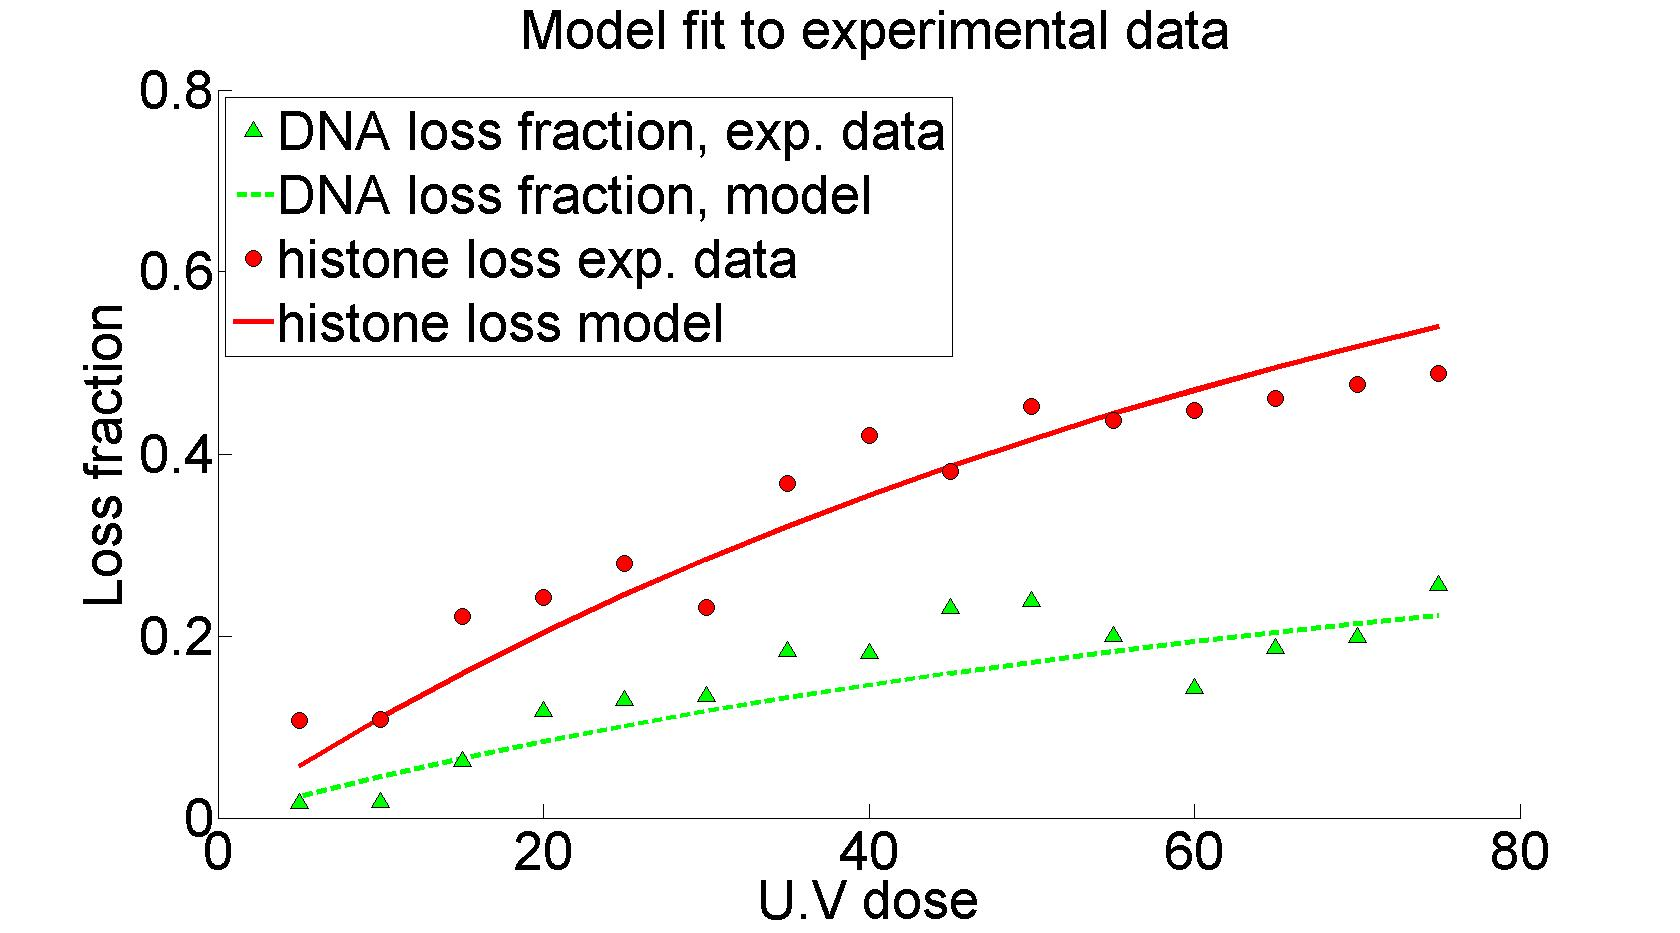
\includegraphics[width=0.5\linewidth, height=0.3\textheight]{histoneAndDnaVsUvDoseModelFit}
\caption{\textbf{Fit of the equation \ref{eq:totalHiostoneLossVsUV} for histone loss (red curve) to the experimental data (red circle). Parameters values obtained were $K_RN_0 =0.7\quad k_rt_s/l=0.007$ resulted in SSE of 0.023. These parameter values were then plugged into equation \ref{eq:dnaLoss} and plotted (green dashed curve) against the experimental data for DNA loss (green circles), resulting in SSE of 0.0208}}
\label{fig:histoneAndDnaVsUvDoseModelFit}
\end{figure}

\subsection{Finding the fraction of nucleosome loss attributed to sliding}
%%%%%%%%%%%%%%%%%%%%%%%%%%%%%%%%%%%%%%%%%%%%%%%%%%%%%%%%%%%

%\beq\label{eq:totalHiostoneLossVsUV} %incorrect
%(N_0-N_15)/N_0 =\frac{h(U)-d(U)}{1-d(U)}.
%\eeq

Using parameters found in subsection \ref{subsection:parameterFit}, we can now calculate the fraction of histones loss attributed to sliding, namely $h(U)-d(U)$.

\begin{figure}[H]
\centering
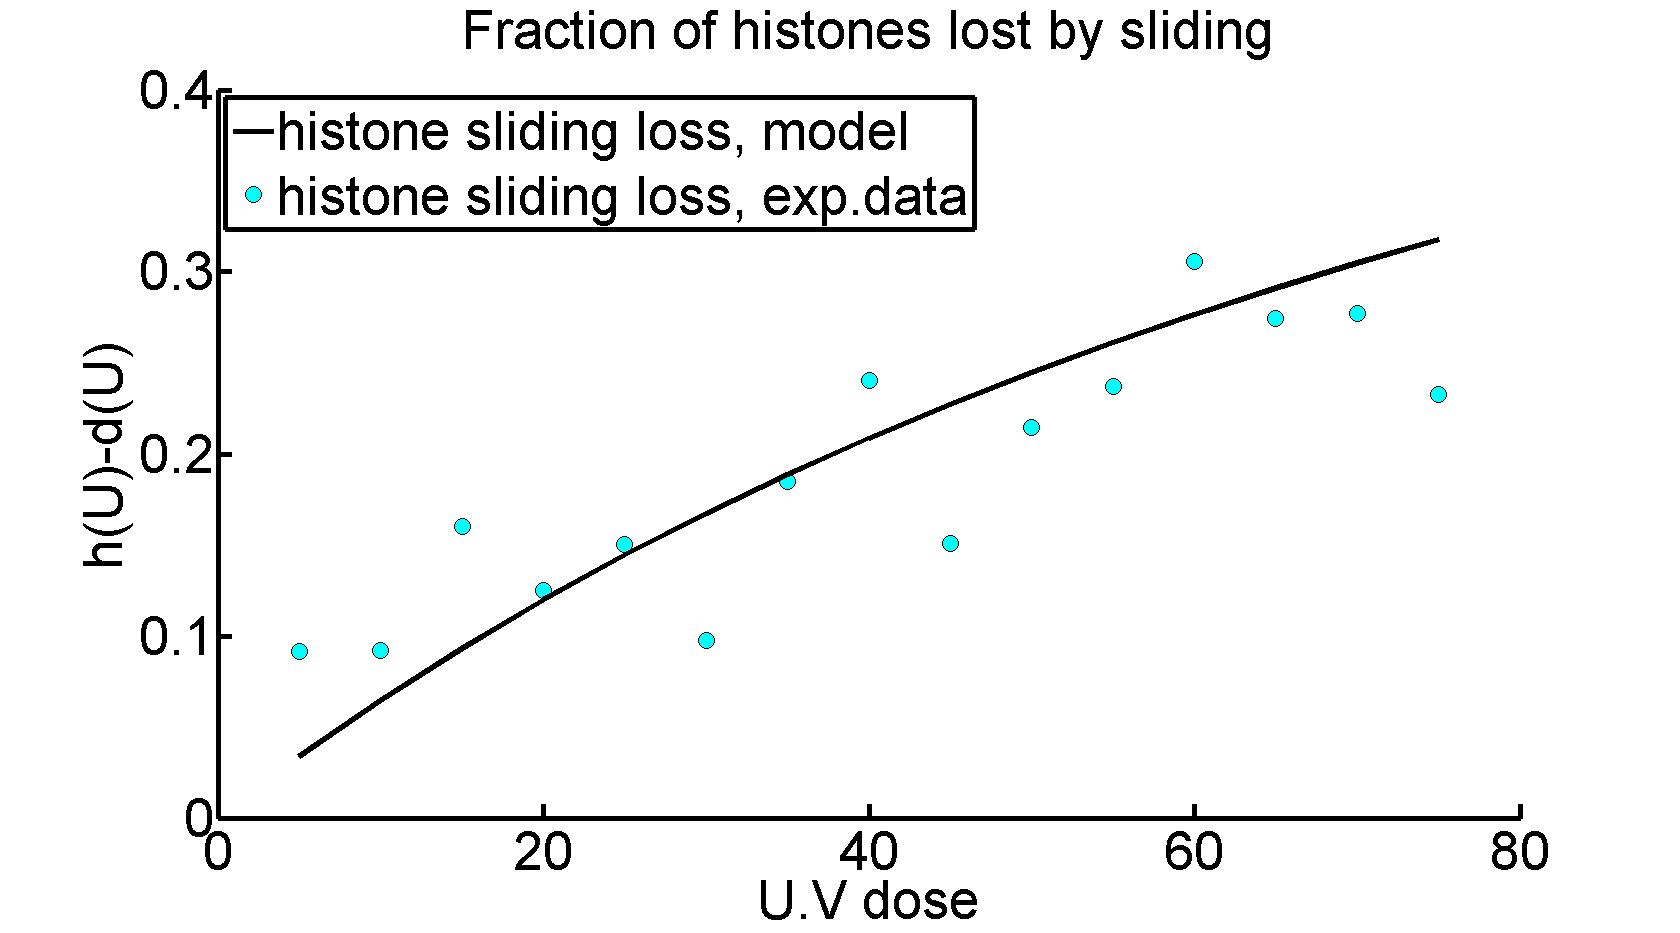
\includegraphics[width=0.5\linewidth, height=0.3\textheight]{hVsUVDoseModelFit01}
\caption{\textbf{The model values for the fraction $h(U)-d( U)$ of histone loss attributed to sliding, plotted against the experimental data}}
\label{fig:hVsUVDoseModelFit01}
\end{figure}

Furthermore, we can calculate the fraction of histone sliding out of the DR, namely $\frac{h(U)-d(U)}{1-d(U)}$. We find a near linear behavior of this quantity, as evident
in Figure \ref{fig:histoneSlideFromDamageRegionComparision}, the qualitative difference between the model and the linear fit is small, in the sense that both capture well the increase in sliding fraction in the UV dose range of the experimental data with near equal variations from experimental data (SSE model = 0.031, SSE linear fit= 0.039).

\begin{figure}[H]
	\centering
	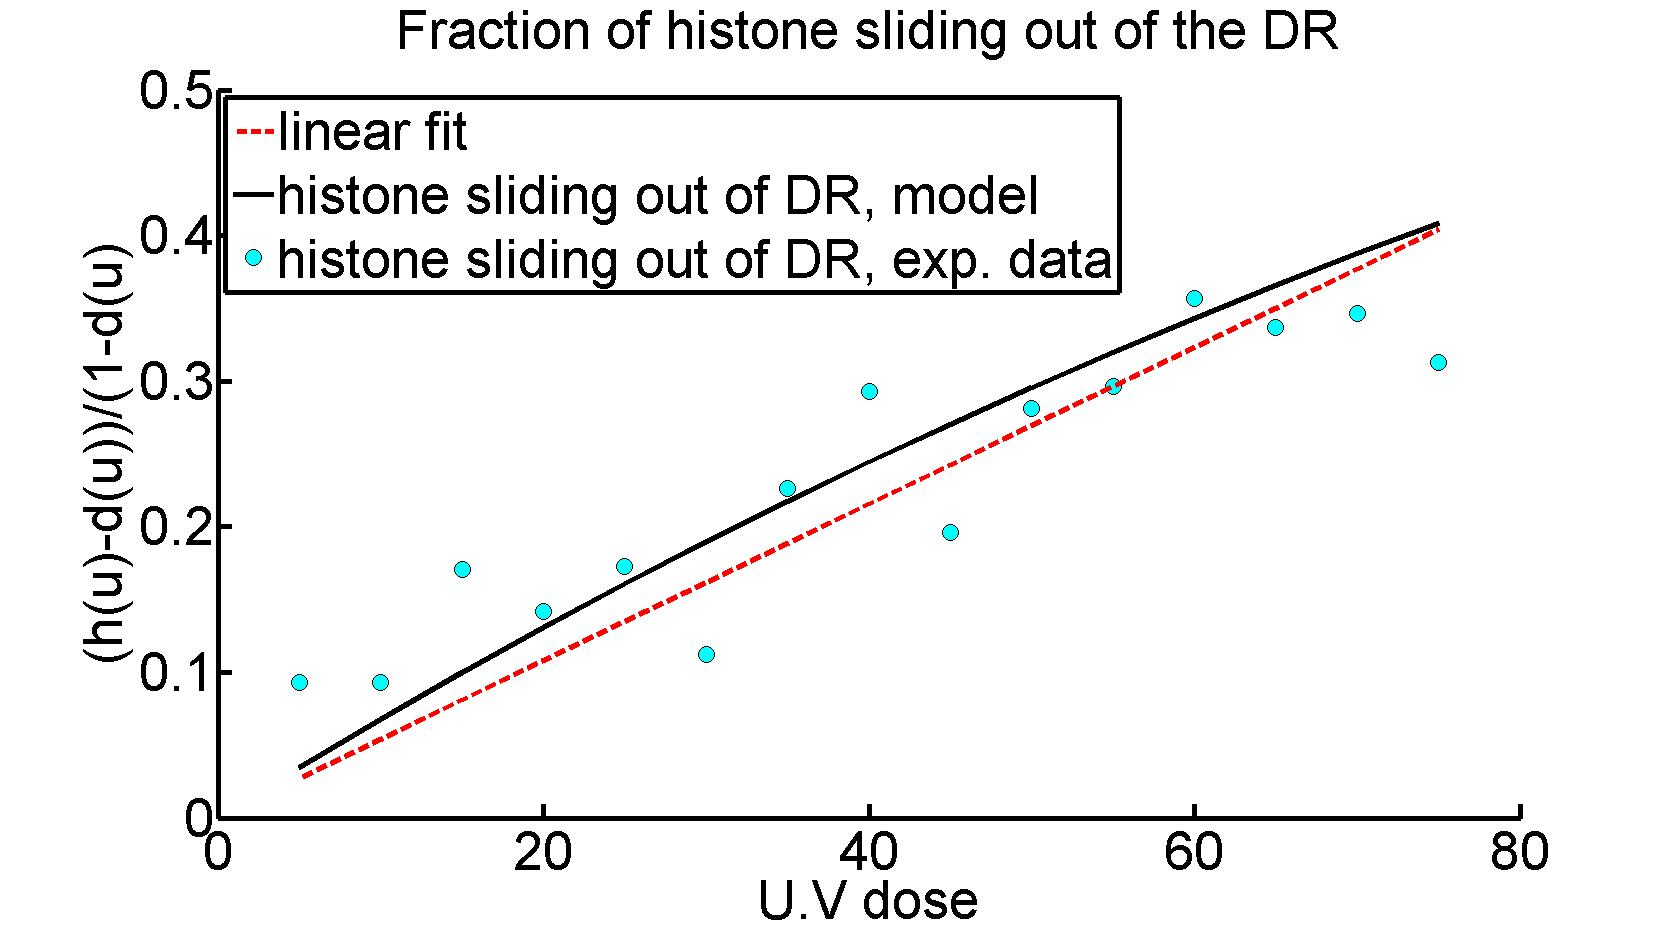
\includegraphics[width=0.7\linewidth, height=0.3\textheight]{histoneSlideFromDamageRegionComparision}
	\caption{\textbf{The fraction of histones lost from the DR due to sliding. The model (black curve) shows a near linear increase in the range of UV dosage tested for the experimental data $(h-d)/(1-d)$. Indeed, the linear fit (dashed red line) shows qualitatively similar behavior to the model, althouth with hight SSE (model =0.031, vs. linear fit=0.039 ) }}
	\label{fig:histoneSlideFromDamageRegionComparision}
\end{figure}

Interestingly, we find that independent of the UV dose, the relative contribution of histone sliding loss to the total histone loss remains a constant of roughly 60\% of the total loss  (Figure \ref{fig:relativeSlidingContribution}). 

\begin{figure}[H]
\centering
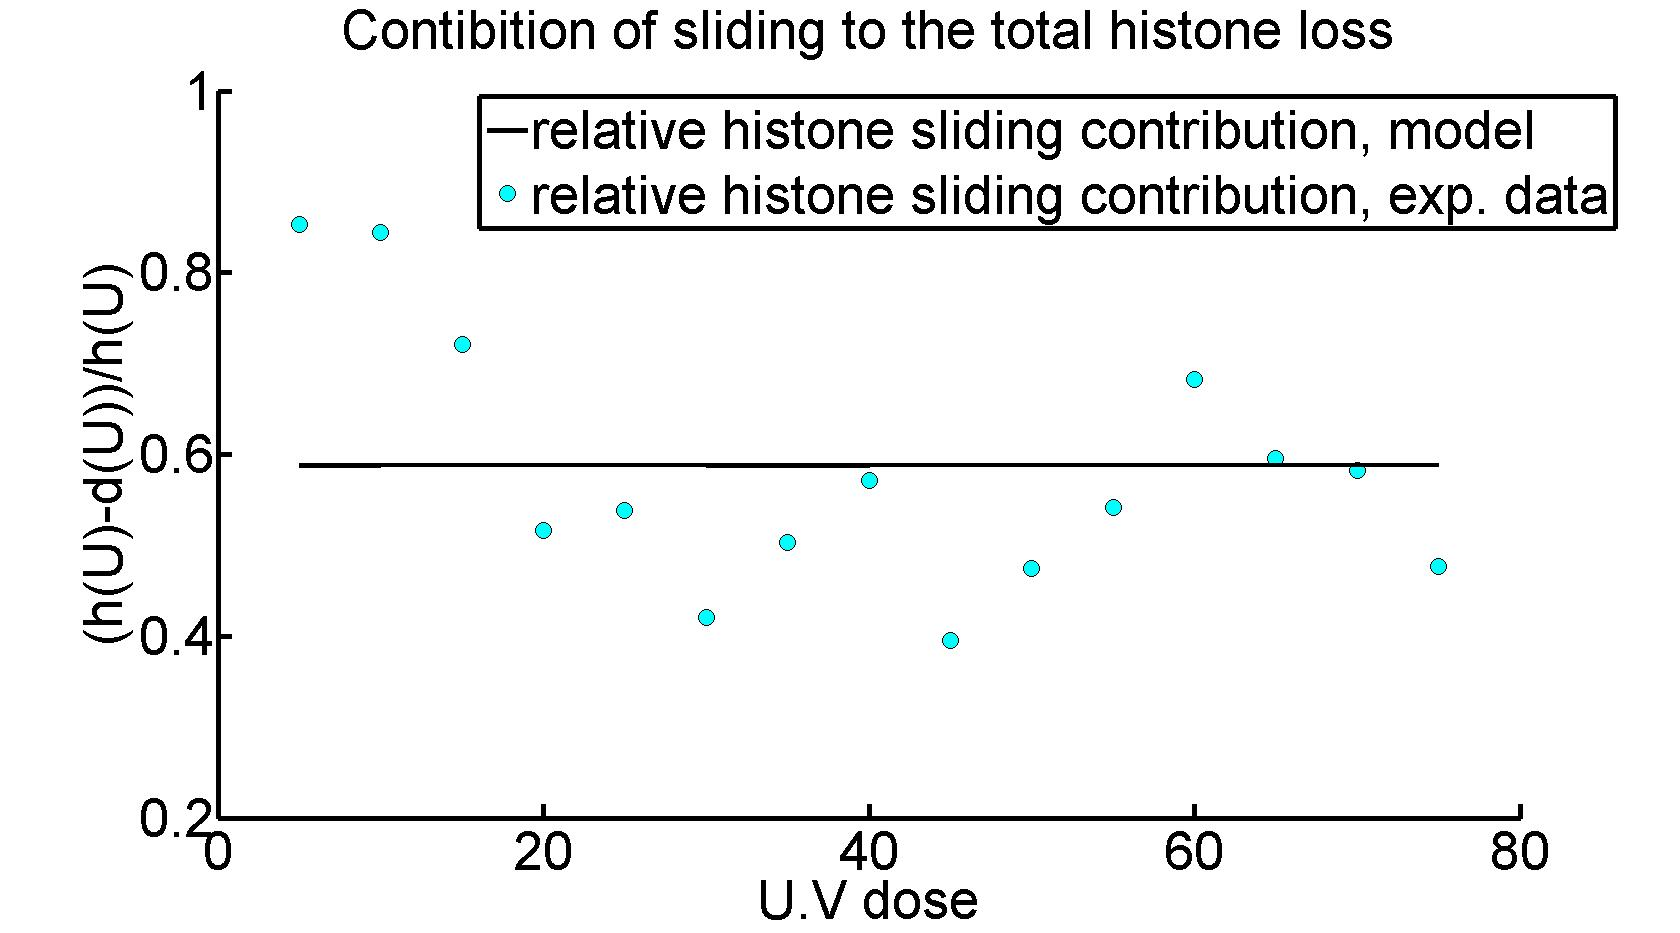
\includegraphics[width=0.5\linewidth, height=0.3\textheight]{relativeSlidingContribution}
\caption{\textbf{The relative contribution of sliding to the total histone loss, $(h(U)-d(U))/h(U)$, is found to be constant according to our model (black line). Indeed, the variations between experimental data (blue circle) and our model shows that the fraction of sliding contribution to the total histone loss can be considered independent of the UV dose}}
\label{fig:relativeSlidingContribution}
\end{figure}

\subsection{Relative contribution of sliding and chromatin opening to the expansion of the DR}\label{subsection:RelativecontibutionOfSlidingAndOpeningToExpansion}

We now turn to calculate the fraction of expansion attributed to both histone sliding and chromatin opening. For this end we use equation \ref{eq:histoneLoss} for the time dependent function of histone loss, and search for the time $\hat{t}$ for which the histone loss fraction reaches 0.6, namely the constant value estimated for $(h(U)-d(U))/h(U)$. In this calculation we set the time to be $t=\kappa t_s$, with $0\leq \kappa\leq 1$. Using expressions \ref{eq:histoneLoss} and \ref{eq:totalHistoneLoss} we solve for $\kappa$ the equation
\beq
0.6h(t_s)=1-\frac{\exp(-\kappa C_1)}{ 1+C_2(1-\exp(-\kappa C_1))}
\eeq
to obtain 
\beq \label{eq:timeFractionForHistoneLoss}
\kappa = -\frac{1}{C_1 U}\ln{\frac{(C_2+1)(1-0.6h(t_s))}{1+C_2 -0.6h(t_s)}}
\eeq
Using $\kappa$ we calculate the relative expansion attributed to sliding by the relation 
\beq \label{eq:relativeSlidingExpansion}
\frac{\alpha(\kappa t_s)}{\alpha (t_s)}
\eeq
The complementary function $1-\frac{\alpha(\kappa t_s)}{\alpha(t_s)}$, is the contribution of chromatin opening to the total expansion of the DR. Plugging \ref{eq:timeFractionForHistoneLoss} into \ref{eq:relativeSlidingExpansion}, we obtain the curve in Figure \ref{fig:histoneAndDNARelativeExpansionContribution}. As can be appreciated from Figure \ref{fig:histoneAndDNARelativeExpansionContribution}, the major contribution to the expansion of the DR comes from the mechanism of histone sliding, which takes up above 80\% for all UV dosages. We interpret the decreasing relative contribution of histone sliding to the expansion as the increase in the need for DNA reorganization with increase in UV dose. With increasing UV dose more DNA is damaged in the IDR, which results in more chromatin opening and eventual loss of DNA and histones from the ROI.

We note that the time dependent histone loss behaves in a near linear fashion independent of  UV dose (data not shown), which allows us to approximate the relative expansion related to histone sliding regardless of the exact time point, but as a function of the total time it takes to lose 60\% of the histones from the ROI. We further note that the mechanism of DNA and histone loss due to chromatin opening contributes to the expansion during histone sliding. However, DNA and histone loss attributed solely to chromatin opening can operate with no sliding. 

\begin{figure}[H]
\centering
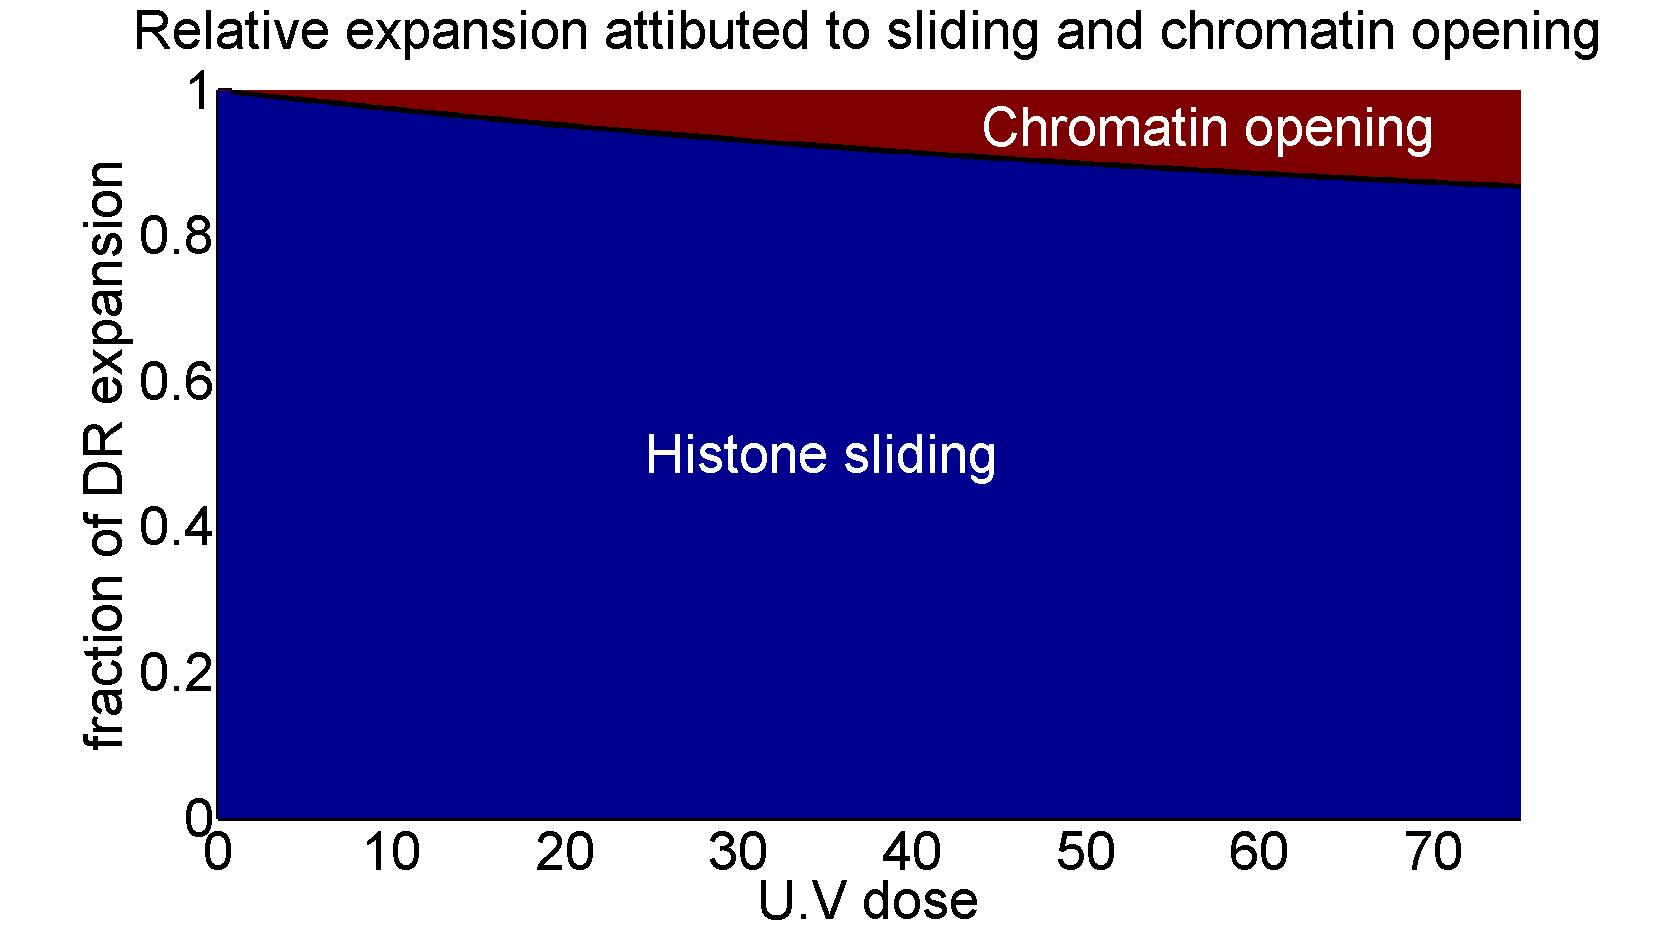
\includegraphics[width=0.5\linewidth, height=0.3\textheight]{histoneAndDNARelativeExpansionContribution}
\caption{\textbf{Relative contribution of histone sliding (blue) and chromatin opening (red) to the total expansion of the DR. Roughly 60\% of the total loss is attributed to histone sliding, independent of the UV dose (Figure \ref{fig:relativeSlidingContribution}), for which the relative contribution for the expansion of the DR is decreasing with UV dose, but remains the main driving force for expansion (above 80\% for all UV dosages). We note that chromatin opening works in parallel to histone sliding. }}
\label{fig:histoneAndDNARelativeExpansionContribution}
\end{figure}



\end{document}

